\documentclass[12pt,titlepage]{article}
\usepackage[margin=1.25in]{geometry}
\usepackage{graphicx,amsmath}

%% Variables definition
\newcommand{\vSubject}{Matematika 3}
\newcommand{\vSubtitle}{Tree}
\newcommand{\vName}{Dicha Zelianivan Arkana}
\newcommand{\vNIM}{2241720002}
\newcommand{\vClass}{2i}
\newcommand{\vDepartment}{Information Technology}
\newcommand{\vStudyProgram}{D4 Informatics Engineering}

%% [START] Tikz related stuff
\usepackage{tikz}
\usetikzlibrary{svg.path,calc,shapes.geometric,shapes.misc}
\tikzstyle{terminator} = [rectangle, draw, text centered, rounded corners = 1em, minimum height=2em]
\tikzstyle{preparation} = [chamfered rectangle, chamfered rectangle sep=0.75em, draw, text centered, minimum height = 2em]
\tikzstyle{process} = [rectangle, draw, text centered, minimum height=2em]
\tikzstyle{decision} = [diamond, aspect=2, draw, text centered, minimum height=2em]
\tikzstyle{data}=[trapezium, draw, text centered, trapezium left angle=60, trapezium right angle=120, minimum height=2em]
\tikzstyle{connector} = [line width=0.25mm,->]
%% [END] Tikz related stuff

%% [START] Fancy header related stuff
\usepackage{fancyhdr}
\pagestyle{fancy}
\setlength{\headheight}{15pt} % compensate fancyhdr style
\fancyhead{}
\fancyfoot{}
\fancyfoot[L]{\thepage}
\fancyfoot[R]{\textit{\vSubject - \vSubtitle}}
\renewcommand{\footrulewidth}{0.4pt}% default is 0pt, overline for footer
%% [END] Fancy header related stuff

%% [START] Custom tabular command related stuff
\usepackage{tabularx}
\newcommand{\details}[2]{
    #1 & #2  \\
}
%% [END] Custom tabular command related stuff

%% [START] Figure related stuff
\newcommand{\image}[3][1]{
    \begin{figure}[h]
        \centering
        \includegraphics[#1]{#2}
        \caption{#3}
        \label{#3}
    \end{figure}
}
%% [END] Figure related stuff

\begin{document}
\begin{titlepage}
    \centering
    \vfill
    {\bfseries\LARGE
        \vSubject\\
        \vskip0.25cm
        \vSubtitle
    }
    \vfill
    
\includegraphics[width=6cm]{images/polinema-logo.png}
    \vfill
    {
        \textbf{Name}\\
        \vName\\
        \vskip0.5cm
        \textbf{NIM}\\
        \vNIM\\
        \vskip0.5cm
        \textbf{Class}\\
        \vClass\\
        \vskip0.5cm
        \textbf{Department}\\
        \vDepartment\\
        \vskip0.5cm
        \textbf{Study Program}\\
        \vStudyProgram
    }
\end{titlepage}

\section*{Task}
\subsection*{Task 1}
Which of the following image is a tree graph?

\begin{figure}[h]
    \centering
    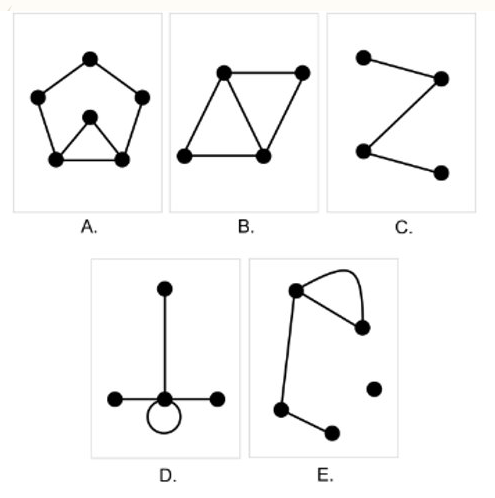
\includegraphics[width=0.5\textwidth]{images/tree-1.png}
\end{figure}

The C and D image are the tree graph because it has no cycle and connected.

\subsection*{Task 2}
Find the minimum spanning tree from the following image with the prim algorithm, continue the table below.

\begin{figure}[h]
    \centering
    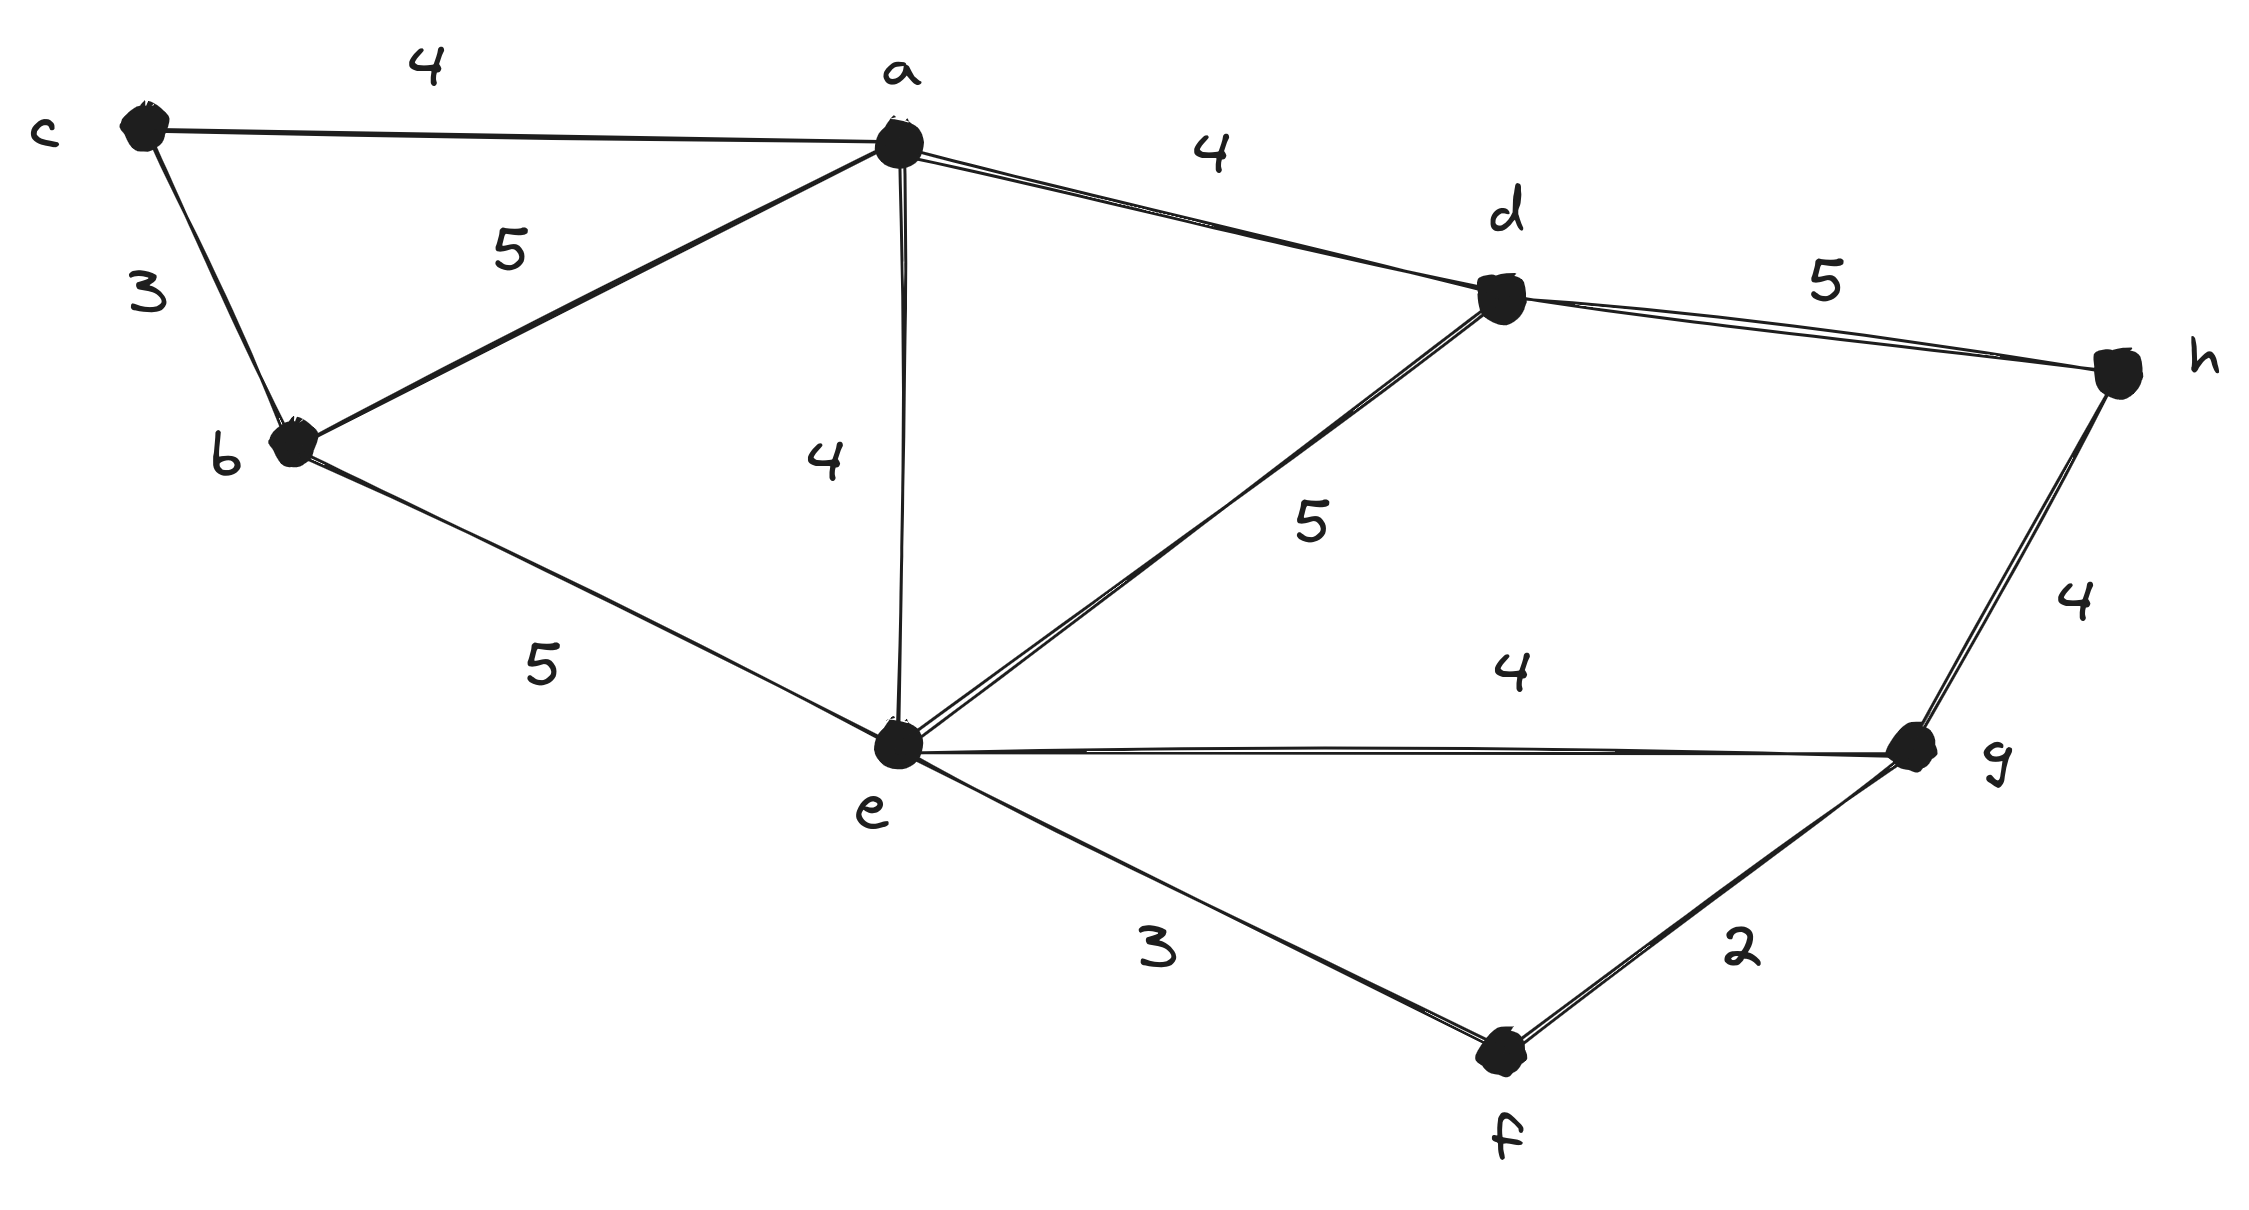
\includegraphics[width=0.5\textwidth]{images/tree-complete.png}
\end{figure}

\begin{table}[h]
    \begin{tabularx}{\textwidth}{|c|c|c|X|}
        \hline
        \textbf{Step} & \textbf{Edge} & \textbf{Weight} & \textbf{MST} \\
        \hline
        1 & (f, g) & 2 & 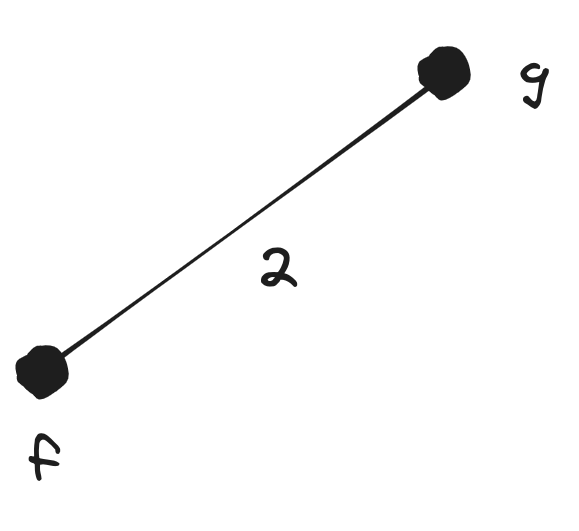
\includegraphics[height=2cm]{./images/tree-f-g.png} \\
        \hline
        2 & (f, e) & 3 & 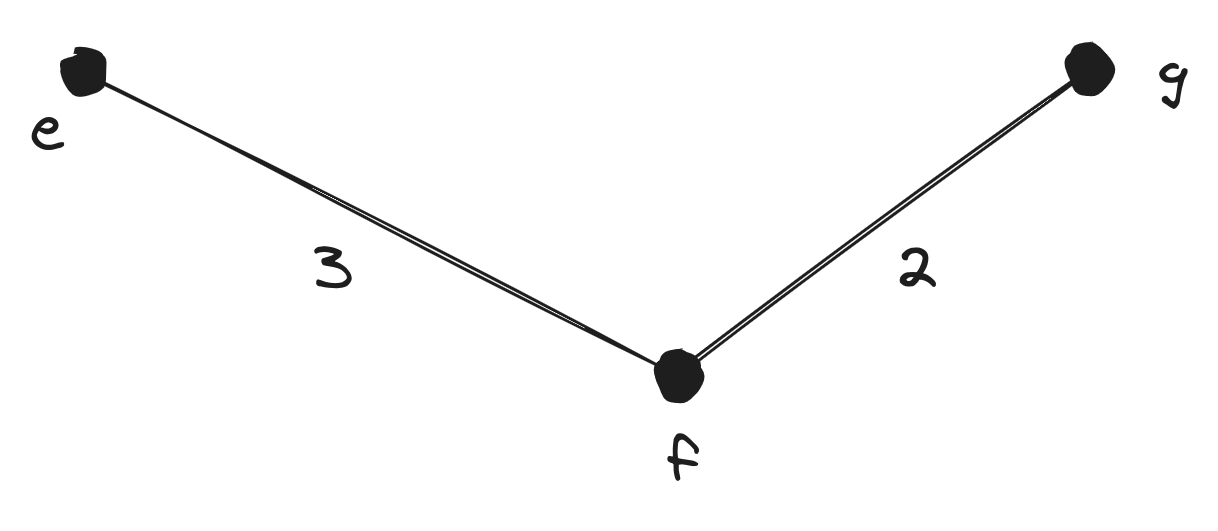
\includegraphics[height=2cm]{./images/tree-f-e.png} \\
        \hline
        3 & (g, h) & 4 & 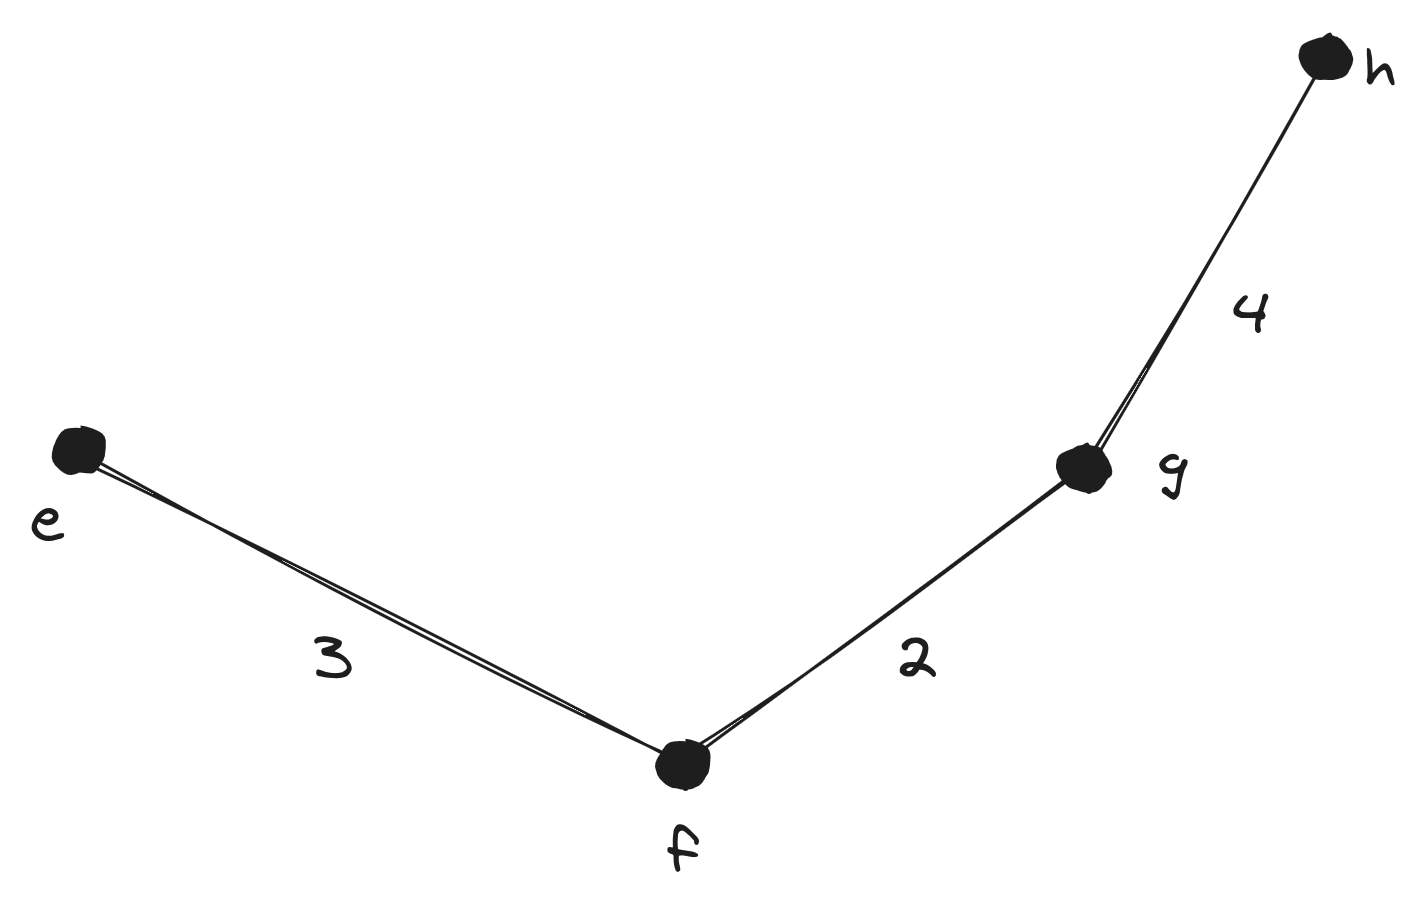
\includegraphics[height=3cm]{./images/tree-g-h.png} \\
        \hline
        4 & (a, e) & 4 & 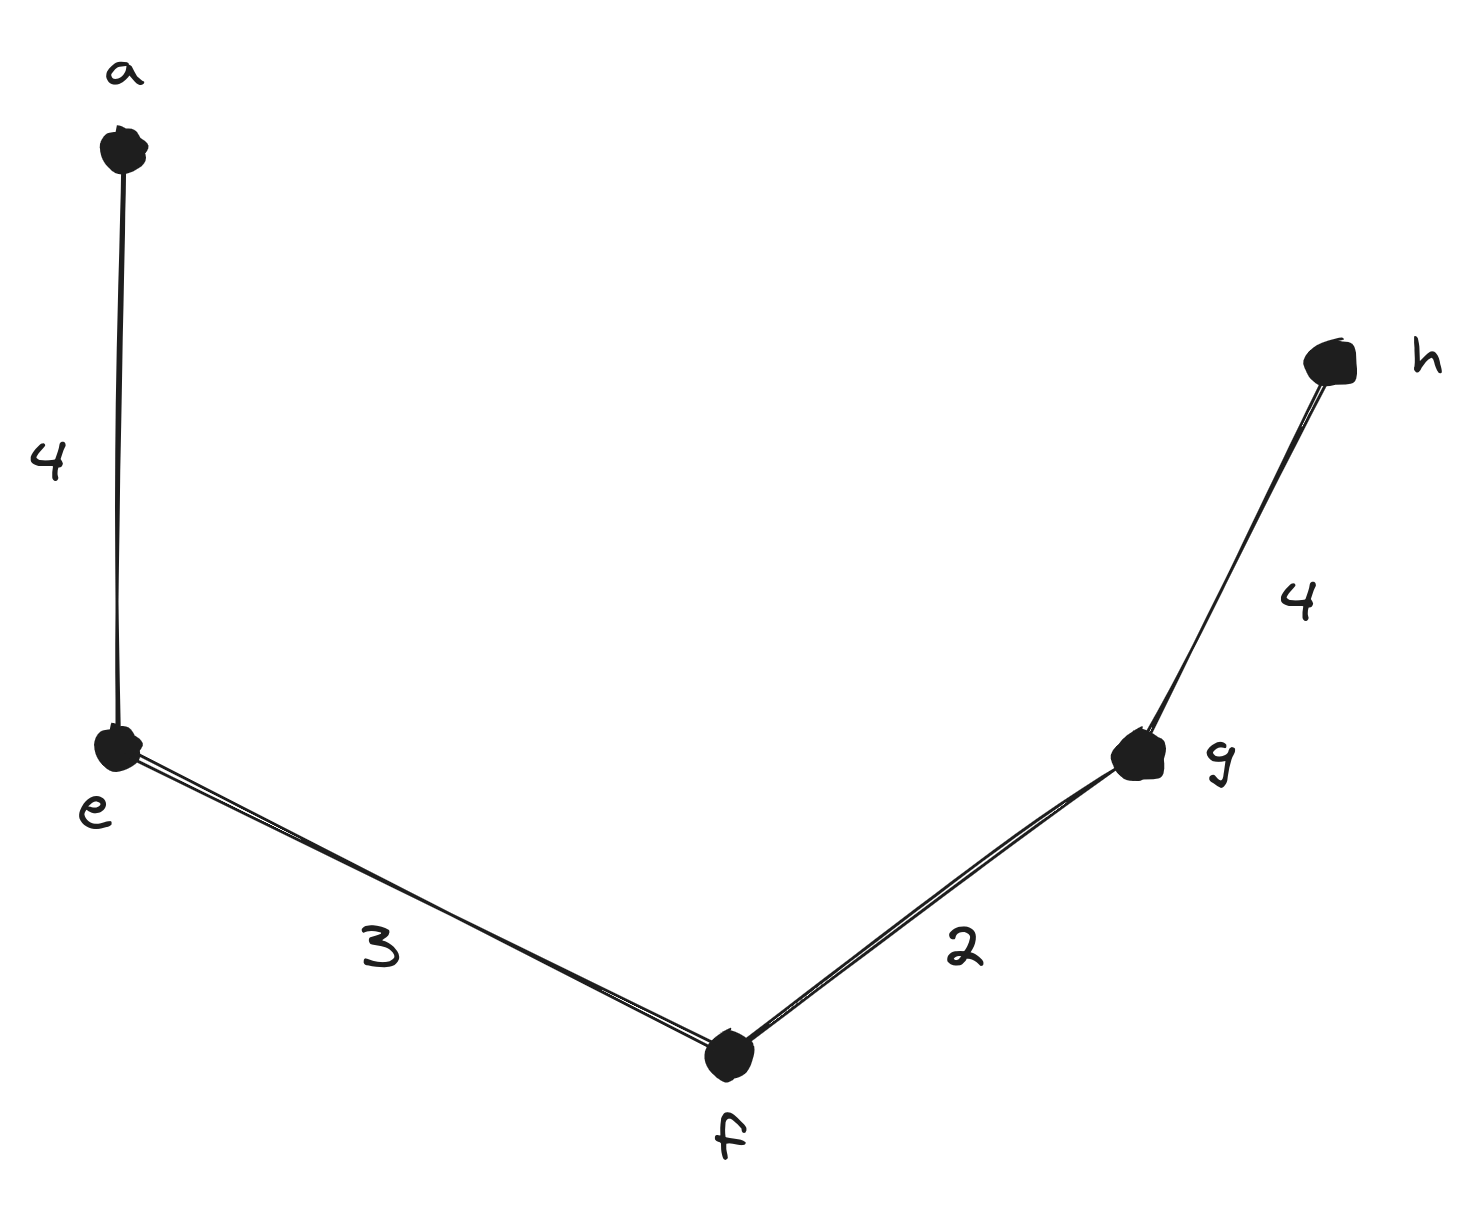
\includegraphics[height=3cm]{./images/tree-e-a.png} \\
        \hline
        5 & (a, d) & 4 & 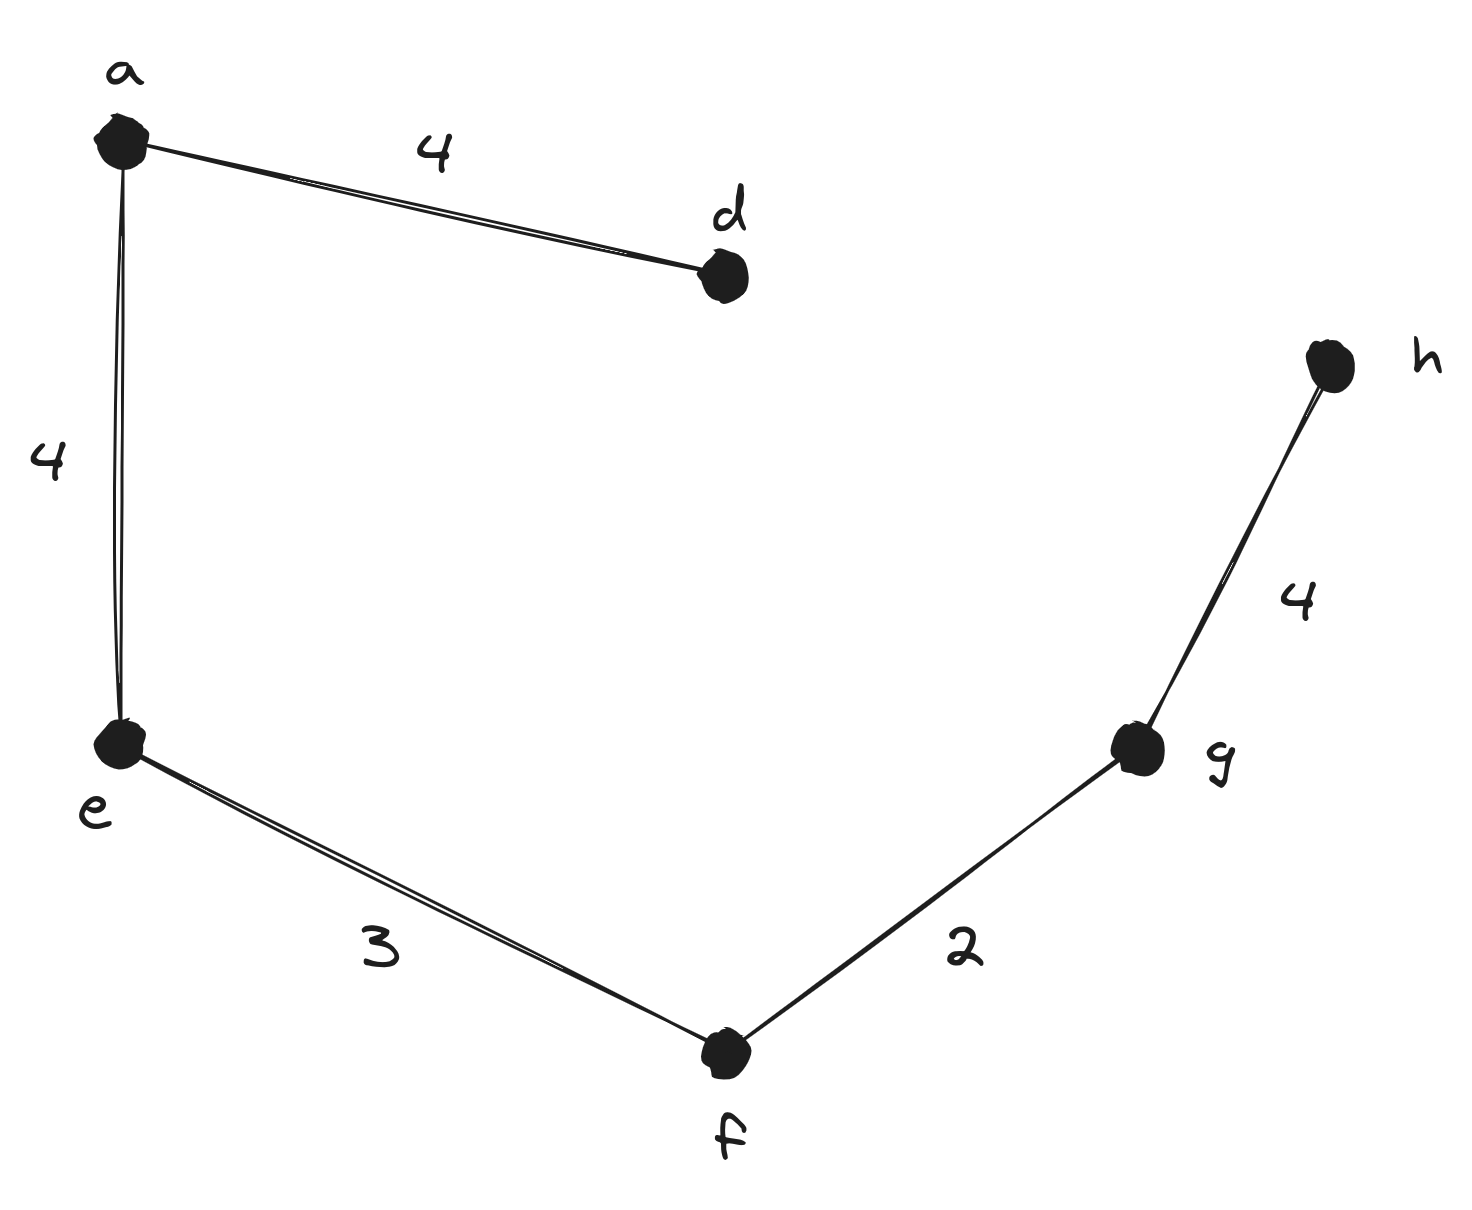
\includegraphics[height=3cm]{./images/tree-a-d.png} \\
        \hline
        6 & (a, c) & 4 & 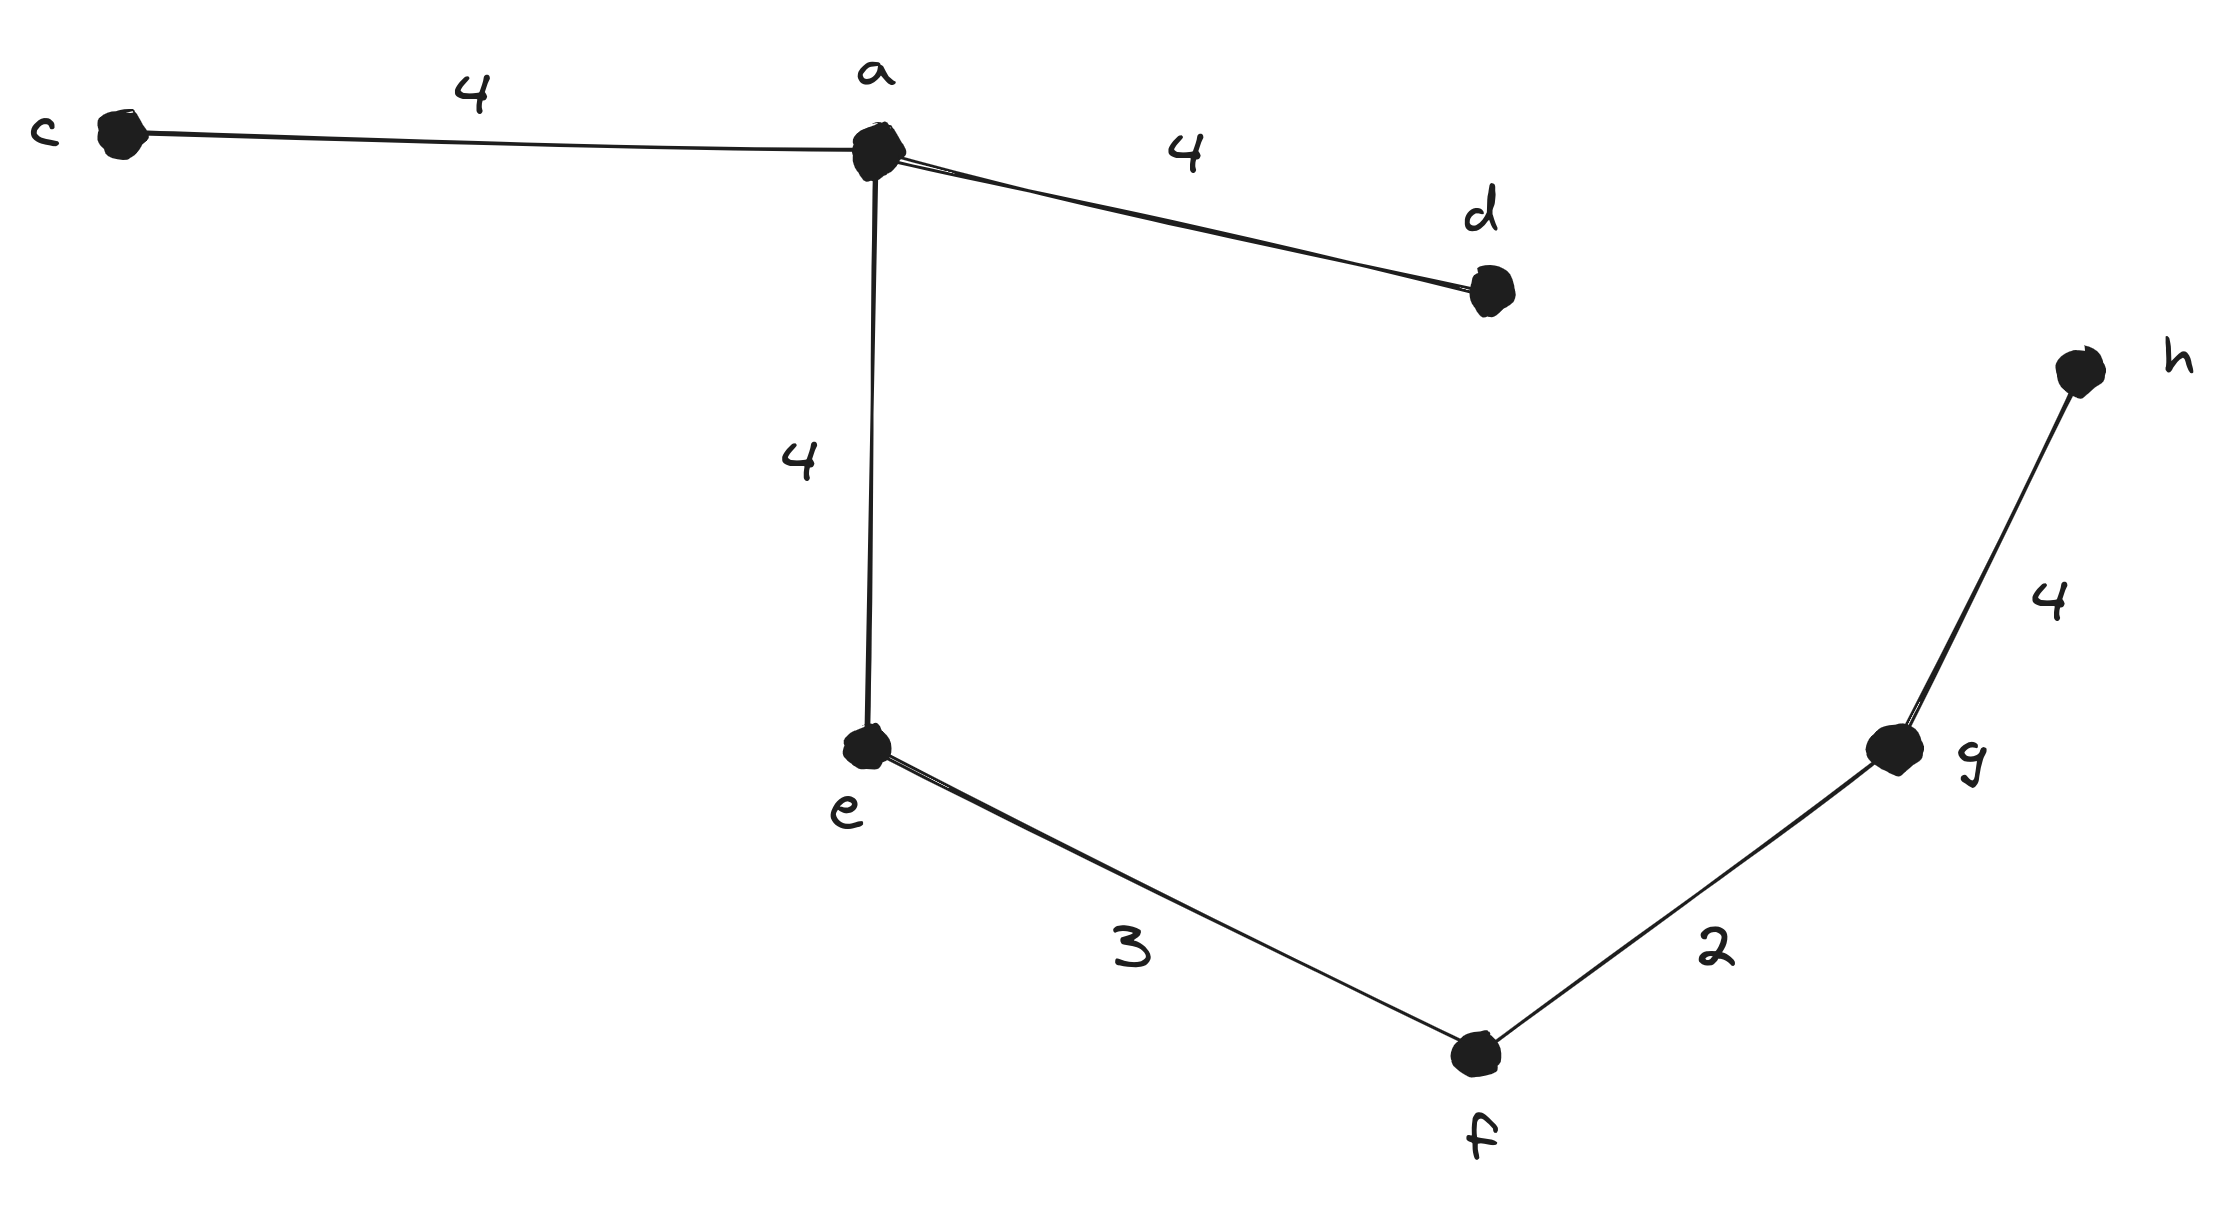
\includegraphics[height=3cm]{./images/tree-a-c.png} \\
        \hline
        7 & (b, c) & 3 & 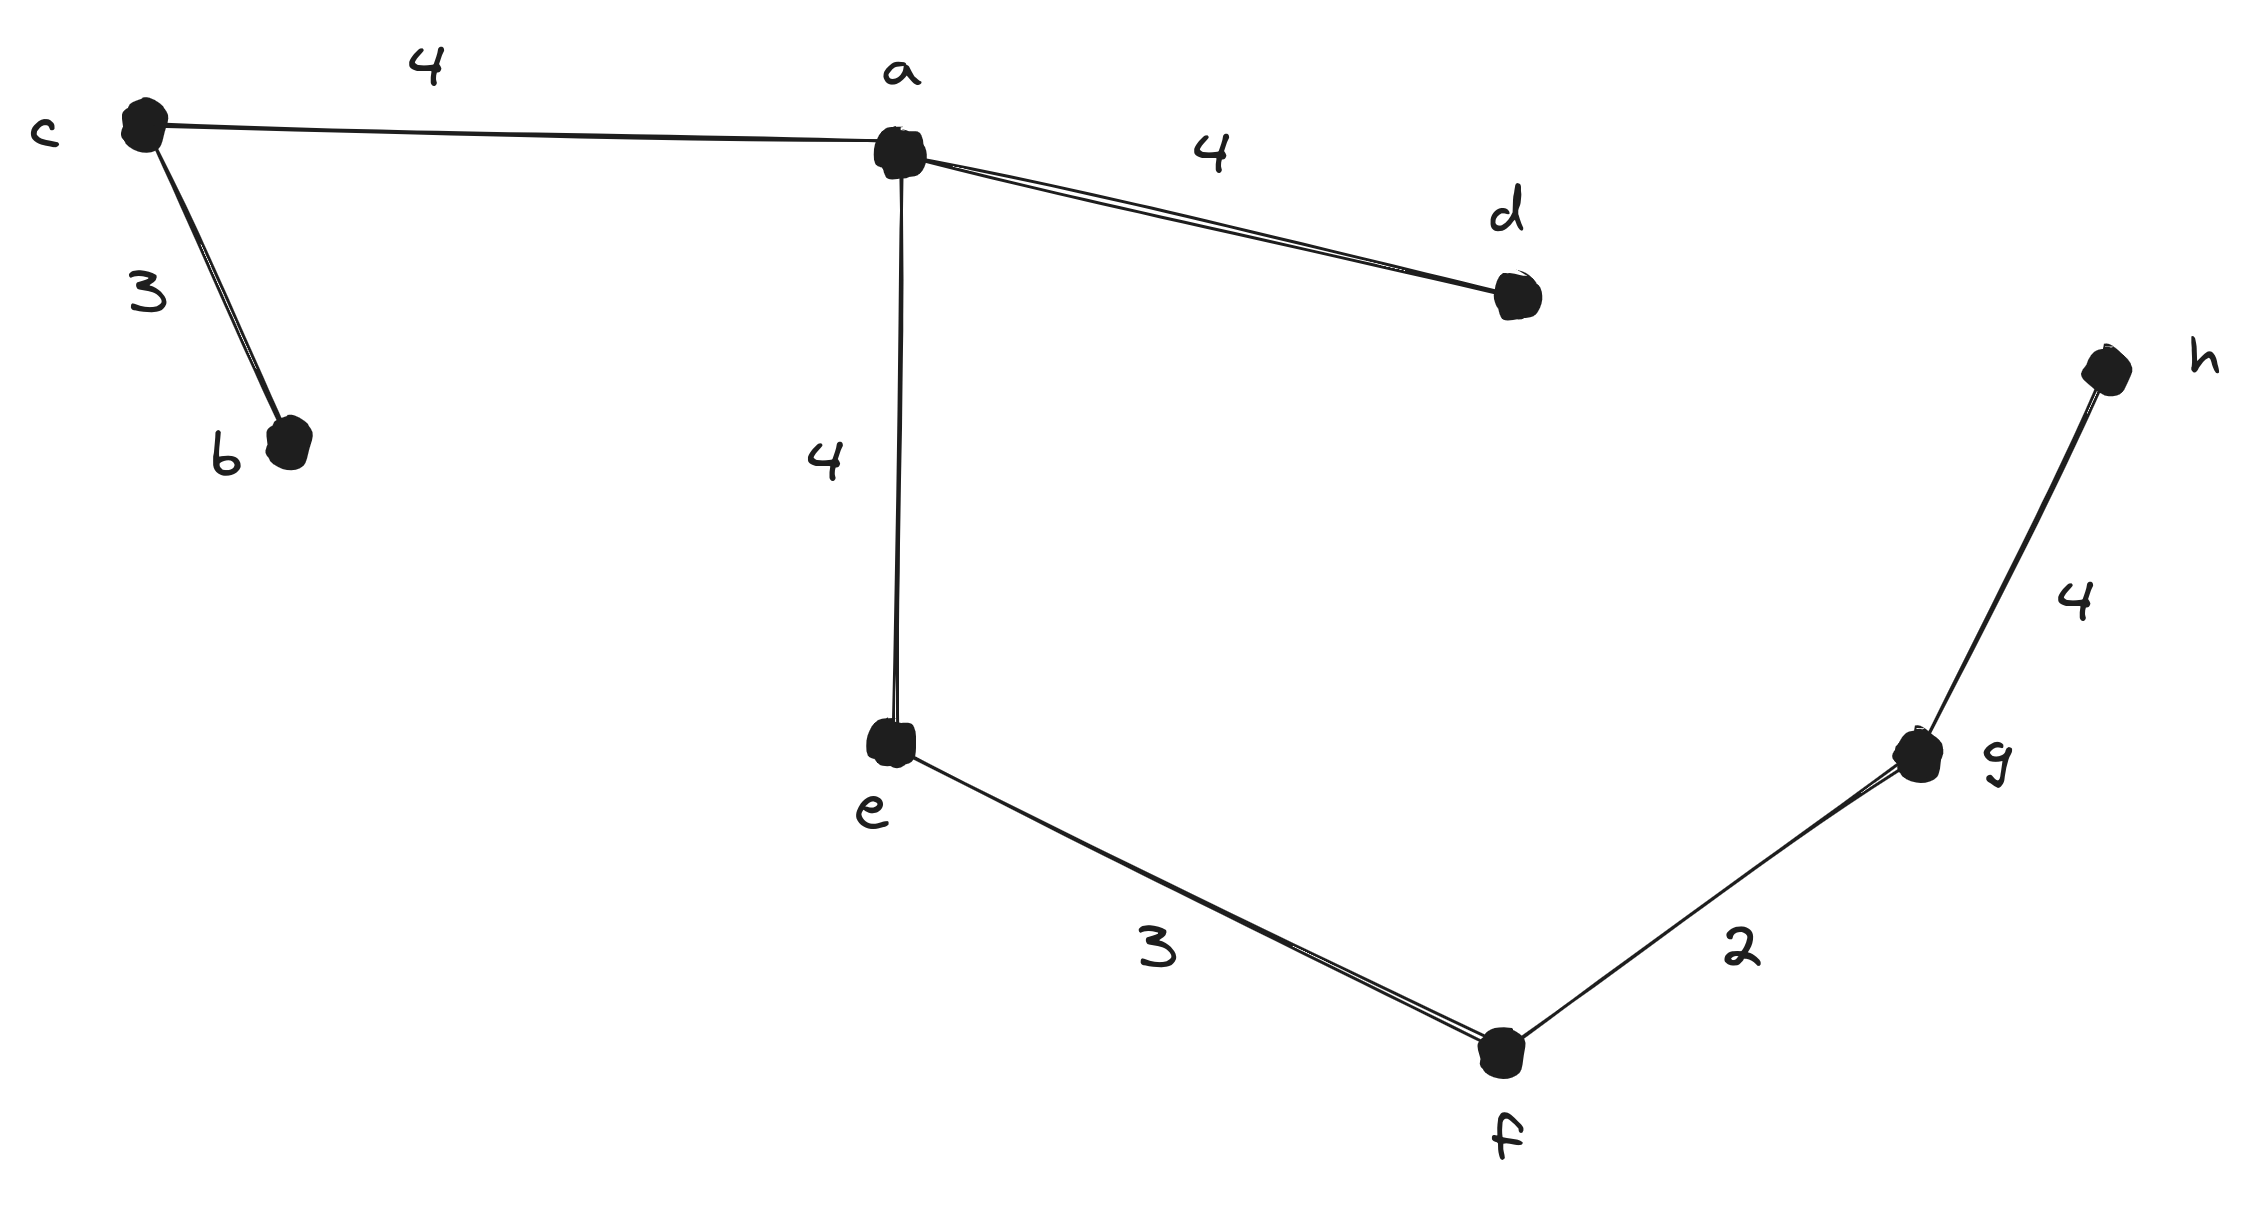
\includegraphics[height=3cm]{./images/tree-c-b.png} \\
        \hline
    \end{tabularx}
\end{table}

\pagebreak

\subsection*{Task 3}
Look for 1 example of a journal application of a Tree / Decision tree and draw a picture of the tree arrangement

\begin{figure}[h]
    \centering
    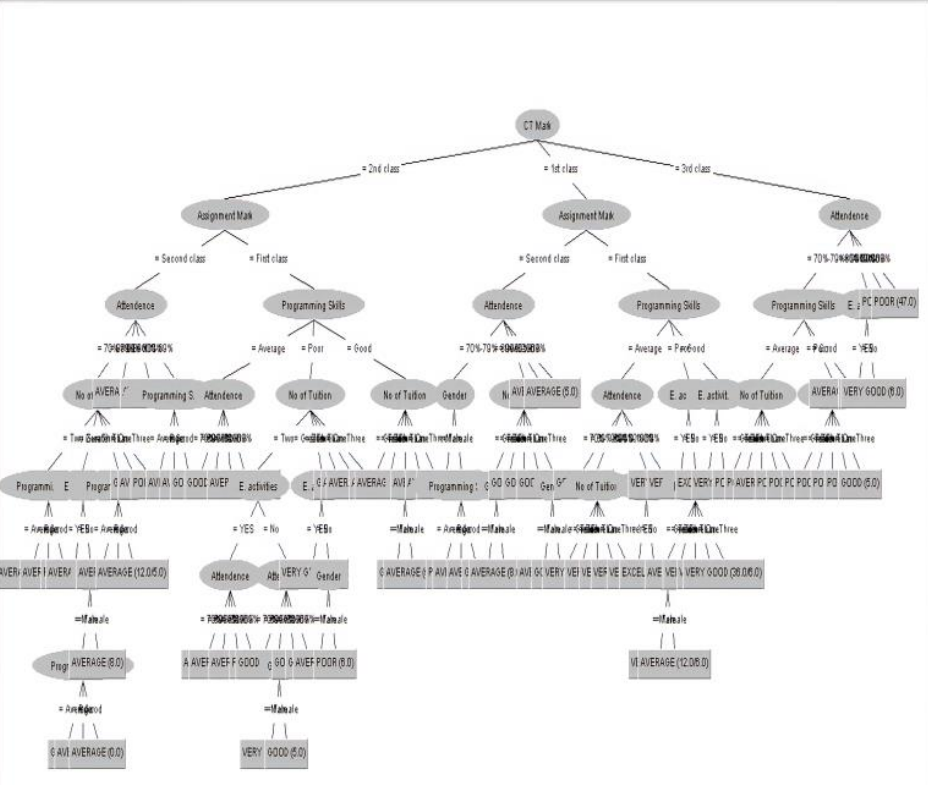
\includegraphics[width=\textwidth]{./images/tree-journal.png}
\end{figure}

\textbf{University Students Result Analysis and Prediction System by Decision Tree Algorithm}
- Md. Imdadul Hoque, Abul kalam Azad, Mohammad Abu Hurayra Tuhin, Zayed Us Salehin

\end{document}

